\def\year{2018}
%File: formatting-instruction.tex
\documentclass[letterpaper]{article}
\usepackage[ruled,vlined,linesnumbered]{algorithm2e}
\usepackage{aaai18}
\usepackage{times}
\usepackage{helvet}
\usepackage{color}
\usepackage{graphicx}
\usepackage{courier}
\usepackage{amsthm}
\usepackage{amsmath}
\usepackage{amssymb}
\usepackage{url}
\usepackage{listings}
\usepackage{multirow}
\usepackage{caption}
\usepackage{subcaption}
\usepackage{numprint}

\newcommand\note[1]{\textcolor{red}{#1}}

\usepackage{adjustbox}
\usepackage{array}

\newcolumntype{R}[2]{%
    >{\adjustbox{angle=#1,lap=\width-(#2)}\bgroup}%
    l%
    <{\egroup}%
}
\newcommand*\rot{\multicolumn{1}{R{45}{1em}}}% no optional argument here, please!

% Defs 
%\newcommand{\public}[1]{\textit{public(#1)}}
%\newcommand{\private}[2]{\textit{private_{#1}(#2)}}
\newcommand{\public}[1]{public(#1)}
\newcommand{\private}[2]{private_{#1}(#2)}

\newcommand{\start}{\ensuremath{*}}
\DeclareMathOperator*{\argmax}{argmax}

\frenchspacing
\setlength{\pdfpagewidth}{8.5in}
\setlength{\pdfpageheight}{11in}

\setlength{\belowcaptionskip}{-10pt}

\pdfinfo{
/Title (MDP-based Cost Sensitive Classification using Decision Trees)
/Author (Guy Shani and Shlomi Maliah)}

\newtheorem{definition}{Definition}
\newtheorem{theorem}{Theorem}
\newcommand\roni[1]{\textcolor{blue}{roni: #1}}
\newcommand\guy[1]{\textcolor{red}{guy: #1}}
\newcommand\cprivacy{object cardinality privacy}
\newcommand\commentout[1]{}

\theoremstyle{definition}
\newtheorem{example}{Example}[section]


\setcounter{secnumdepth}{2}

 \begin{document}
% The file aaai.sty is the style file for AAAI Press 
% proceedings, working notes, and technical reports.
%
% Joerg: slightly adapted title, more close to previous nomenclature
%
\title{MDP-based Cost Sensitive Classification using Decision Trees}
%\title{Partially Observable Contingent Planning for Penetration Testing}

\author{Shlomi Maliah \and Guy Shani \\\\
Software and Information Systems Engineering\\
Ben Gurion University, Israel \\
shlomima@post.bgu.ac.il, shanigu@bgu.ac.il
}

\maketitle
\begin{abstract}
\begin{quote}
In classification, an algorithm learns to classify a given instance based on a set of observed attribute values. In many real world cases testing the value of an attribute incurs a cost. Furthermore, there can also be a cost associated with the misclassification of an instance. Cost sensitive classification attempts to minimize the expected cost of classification, by deciding after each observed attribute value, which attribute to measure next. In this paper we suggest Markov Decision Processes as a modeling tool for cost sensitive classification. We construct standard decision trees over all attribute subsets, and the leaves of these trees become the state space of our MDP. At each phase we decide on the next attribute to measure, balancing the cost of the measurement and the classification accuracy. We compare our approach to a set of previous approaches, showing our approach to work better for a range of misclassification costs.

\end{quote}
\end{abstract}


\section{Introduction}

Classification is the task of identifying the class of an instance based on a set of observed attributes. For example, we may conduct a set of tests for a patient to properly identify her condition, applying an appropriate treatment for that condition. In many cases some tests, such as measuring temperature and blood pressure are easy to conduct and incur little cost, while other tests such as gene profiling are much more costly. On the other hand, costly tests are often more informative than blood pressure, and can be more useful for diagnosis. In such cases it may be reasonable to collect measurements in an incremental manner, deciding on the next test after observing the results of the previous test.

In addition, in many applications there is a cost associated with an error on the final classification decision. In the diagnosis example above, an error in classification may cause the doctors to apply a wrong treatment, which may be both costly in hospital resources, as well as damaging to the patient. There are hence two different costs that must be considered ---  a cost for measuring the value of a attribute, and the cost of misclassification. 

Classical classification algorithms ignore these costs, focusing on measuring the value of attributes that provide better accuracy. In many cases better accuracy results implicitly in reduced misclassification cost.
Cost sensitive classification \cite{elkan2001foundations,turney1995cost,LomaxV13}, on the other hand, takes costs directly into consideration.

For example, several researchers suggested to modify the splitting criterion of standard decision tree algorithms, such as C4.5, to take into account costs~\cite{CS-IDS3,IDX,EG2}. Turney \shortcite{turney1995cost} used a genetic algorithm to construct a decision tree, taking into account not only immediate costs, but also future costs. 
%Lomax and Vadera \cite{LomaxVS12} suggested a reinforcement learning approach based on the multi-armed bandit problem...

In this paper we suggest Markov Decision Process (MDP) \cite{Bellman,Puterman} as a useful tool for modeling cost sensitive classification. MDPs allow a classifier to choose which attribute to measure next taking into consideration the expected future sum of costs. MDPs inherently take into consideration future actions, rather than considering only the immediate, myopic gain.

We construct a set of decision trees, over all attribute subsets. These decision trees are learned in the standard manner, ignoring all costs, where each node in the tree is associated with an attribute to measure, and each outgoing edge is associated with a constraint over the observed value for that attribute. Leaves are associated with a final classification decision. The state space of our MDP is the set of leaves of all trees.
When classifying the MDP state conforms to a single leaf in one of the trees, based on the set of attributes values that were observed thus far.
The available MDP actions are to select an additional attribute to test, transitioning to a leaf in other tree, or to classify based on the known attributes. 

After choosing an attribute to measure based on the MDP policy, we transition to a new leaf in another tree given the observed attribute value. The cost of attribute measurement actions are the costs of the tests, and the costs for the final classification decision are the misclassification costs.

Even though we construct multiple decision trees, we do not propose an ensemble approach \cite{banfield2007comparison}. Our approach can be described as constructing a single cost sensitive decision tree from multiple accuracy driven decision trees.

We provide experiments over a set of benchmarks \cite{LomaxV13} showing that our MDP approach scales well over these benchmarks. We provide a set of experiments when varying the cost of misclassification. When the misclassification cost is very high, one will query all available attributes that provide useful information before making a decision. When the misclassification cost is very low, it is often better to make a decision based on the priors without paying the cost of measuring any attribute. We show that for a range of symmetric and asymmetric misclassification costs between these two extremes, our MDP approach outperforms all other methods. 

\section{Background}

We now briefly review relevant background --- decision trees, cost-sensitive classification, and MDPs.

\subsection{Decision Trees}

In classification, given an instance that specifies values for a set of attributes, the classifier must predict a class for that instance. Decision trees are perhaps one of the most popular classification model in machine learning literature, due to their predictive power, as well as their readability. The nodes of the tree are labeled by an attribute. The outgoing edges from a node labeled by an attribute $a$ are labeled by the various possible values of $a$. The leaves are labeled by a class name.

To classify a new instance, one starts at the root, and traverses the tree towards one of the leaves. At each node labeled by an attribute we observe the value of that attribute in the current example, and traverse the edge corresponding to that value. Upon reaching a leaf we classify the instance to the class associated with that leaf.

Classical decision tree induction algorithms, such as ID3 and C4.5, construct a decision tree incrementally, given a population of example instances labeled by known classes. The algorithms start with the entire population and select an attribute that would split the population into different groups, such that the split maximizes some criteria. Typical criteria for preferring one attribute over another can be the information gain or the gain ratio. These algorithms take a greedy approach, choosing the attribute that splits the population best in a single step, ignoring future splits.


\subsection{Cost-sensitive Decision Tree Learning}

Classical classification algorithms assume that when given a new instance to classify, the values of all attributes are already known. This is identical to the case where the values can be acquired online, while classifying, incurring no additional cost. In addition, classical algorithms assume that all classification errors have an identical penalty.

These two assumptions are often invalid in many real world problems, such as sensor activation in cellphones, car failure diagnosis, and medical diagnosis. For example, in medical classification problems \cite{turney1995cost}, the patient diagnosis typically involves a sequence of medical tests. As the tests are costly both in terms of resources (money and time), as well as in inconvenience or even damage to the patient, the goal is to reduce these costs prior to a successful classification. A typical diagnosis process performs tests sequentially, and after observing the results of a test, makes a decision to classify, or to conduct another test. 

\commentout{
It is often the case that less costly tests are also less informative. Hence, a simple escalation strategy starts with the simplest and least informative tests and then moves to more costly tests if need be. 
}
In some cases test costs are not independent, that is, the cost for testing two attributes is lower than the sum of costs of testing each independently. For example, in medical diagnosis, there is a cost associated with extracting a blood sample, but once a blood sample has been extracted, testing additional properties of the blood may not require another sample, and thus has a reduced cost.

It is also natural in such problems to define a cost for misclassification, such as diagnosing the wrong disease, or diagnosing a disease in a healthy person. These misclassifications may result in unneeded expensive treatments. Also, misclassifying a sick patient as healthy may result in serious damage to the  patient. One can also assign a reward for the correct classification of a disease, corresponding to the improvement in the quality of life. Different misclassifications may incur different costs, and different correct classifications may incur different rewards.

Given these two types of costs, it is more reasonable to measure the expected classification cost, rather than the accuracy of the model. Classical classification algorithms that ignore these costs may result in relatively high expected costs. One can adapt arbitrary classification algorithms to be cost sensitive \cite{zadrozny2003cost,domingos1999metacost}. Alternatively, one can construct a cost-sensitive algorithm directly, as we do.


Early cost-sensitive decision tree induction algorithms, such as CS-ID3, IDX, and EG2 take a greedy approach, choosing an attribute given the myopic expected test cost and gain. ICET \cite{turney1995cost} uses a genetic algorithm to learn a decision tree that minimizes the expected cost. Genetic algorithms, as any local search, tend to achieve a local minima, and may hence produce suboptimal classifiers. MetaCost \cite{domingos1999metacost} uses bagging to construct several decision trees over different samples of the data, relabeling examples to their minimal cost class, and then retraining.

Lomax and Vadera \cite{LomaxV11} conduct a comprehensive comparison of cost-sensitive, showing that Turney's ICET is still among the best preforming algorithms, and that IDX \cite{IDX} also preforms well.

We take a maximizing approach, where positive rewards represent desirable outcomes, and negative rewards represent costs and undesirable outcomes, and the goal of the classifier is to maximize the expected reward, rather than minimize the expected cost of classification.
More explicitly, we assume a negative reward (cost) $r_{a|P}$ for testing the value of an attribute $a$ given the set of already tested attributes $P$, and a negative reward $r_{c,c'}$ for misclassifying an example of class $c'$ as class $c$, and a positive reward $r_{c,c}$ for correctly classifying an example of class $c$. 


\subsection{Markov Decision Processes}

A Markov decision process (MDP) \cite{Bellman,Puterman} is a decision making algorithms, designed to take into account future decision while deciding on the next action. Formally an MDP is a tuple $\langle S,A,tr,R,H \rangle$ where $S$ is a set of states, $A$ is a set of actions, $tr$ is a transition function, $R$ is a reward function, and $H$ is the planning horizon --- the maximal amount of steps before the execution terminates.

The state space $S$ models all the relevant features for making a decision. The system is always at exactly one state, and this state is known to the decision maker. The action set $A$ models the actions that are available to the decision maker. At each phase the decision maker observes the current state, and decides on an action. The system then transitions to a new state, and the process is repeated.

The $tr$ function models stochastic state transitions, that is, $tr(s,a,s')=pr(s'|s,a)$ is the probability of transitioning to state $s'$ given that action $a$ was executed at state $s$. We assume the Markovian property, where only the current state influences the transition, i.e., $pr(s_{t+1}|s_0,a_0,s_1,a_1,...,s_{t-1},a_{t-1})=pr(s_{t+1}|s_{t-1},a_{t-1})$.
The reward function $R(s,a)$ models desirable outcomes, as well as action costs.
%\footnote{Other reward structures, such as $R(s)$ or $R(s,a)$ are more popular in literature, but this structure best fits our goals.}. 
A positive reward is given for a successful outcome, such as a correct classification, while a negative reward is used to denote either undesirable outcomes (e.g. misclassification), or action costs (e.g. test costs). Given the Markovian property, rewards depend solely on the action and the state prior to the action, ignoring previous states and actions.


A solution to an MDP is typically expressed as a policy $\pi:S\rightarrow A$ --- a mapping from states to actions. An optimal policy maximizes the expected sum of rewards: $\sum_{i=0..H} r_i$. The value iteration algorithm computes a value function $V:S \rightarrow R$, assigning a value to a state, modeling the expected sum of rewards from that state following an optimal policy.

One can compute a value function iteratively using the Bellman backup \cite{Bellman}:
{\footnotesize
\begin{eqnarray}
V_1(s)&=&\max_a R(s,a)\\
Q_{i+1}(s,a)&=&R(s,a) + \sum_{s' \in S}tr(s,a,s') V_i(s')\\
V_{i+1}(s)&=& \max_{a \in A}  Q_{i+1}(s,a)
\end{eqnarray}
}
where $V_i$ models the expected sum of rewards with $i$ steps to go. Given cyclic transitions value iteration eventually converges, 
%that is, there exists $i$ such that for every $j>i$, $\forall s \in S, |V_{j}(s)-V_i(s)| < \epsilon$. 
but for acyclic transitions, computing values in reversed topological order requires only a single iteration.
Given a value function $V$ we can define a policy:
{\footnotesize
\begin{equation}
\pi(s)=argmax_{a \in A} R(s,a) + \sum_{s' \in S} tr(s,a,s') V(s')
\end{equation}
}
mapping each state to an action to execute.

MDPs have been previously suggested for the related task of dynamic feature selection \cite{he2012cost}, where the goal is to collect a relatively small number of features to increase classification speed.

\subsection{Reinforcement Learning}

When the MDP parameters, the transitions and the rewards, are unknown, one cannot use value iteration directly. Computing a policy under unknown model parameters is typically known as reinforcement learning (RL)\cite{sutton1998reinforcement}. There are two main approaches to RL; In model-based RL, the model parameters are learned from the data, allowing us to use value iteration. In model-free RL the value function is computed directly without learning the model parameters first. Perhaps the most popular model-free method is $Q$-learning \cite{watkins1992q}, where after executing an action $a$, at state $s$, receiving a reward $r$ and transitioning to state $s'$, the value function is updated:
\begin{equation}
Q(s,a) = (1-\alpha) \cdot Q(s,a) + \alpha \cdot (r + \gamma \max_a Q(s',a))
\end{equation}
$Q(s,a)$ is typically called the $Q$ function. 


\section{MDP-based Classification}

We now describe our classification method, which uses an MDP to decide on the next attribute to test, or which class to classify an example. Our method uses a set of decision trees, each over a different subset of attributes. During classification, at each step there is a single active tree, corresponding to the set of already observed attributes, and a single active leaf in that tree, defining the current MDP state. The MDP can decide to transition to another tree and leaf by testing the value of another attributes, or classify the current example.

Let $\mathcal{A} = \{a_1,...,a_n\}$ be the set of attributes, and let $\mathcal{C} = \{c_1,c_2,...,c_m\}$ be the set of classes of the current classification problem. We begin by learning a decision tree for every subset of $\mathcal{A}$, including the empty set. The decision trees are constructed using the standard C4.5 algorithm \cite{quinlan2014c4}. When constructing the trees we maintain in each leaf $l$ of every tree the set of examples $E_l$ that were associated with this leaf during learning.

In cases where there are too many attributes to construct decision trees for all subsets, and some attributes are significantly less costly than others, we can reduce the construction costs by assuming that the less costly attributes are always tested. Let $\mathcal{A}_1 \subset \mathcal{A}$ be the set of costly attributes, and $\mathcal{A}_2 \subset \mathcal{A}$ be the set of low cost attributes, such that $\mathcal{A}_1 \cup \mathcal{A}_2 = \mathcal{A}, \mathcal{A}_1 \cap \mathcal{A}_2 = \emptyset$. For each subset $P \subset \mathcal{A}_1$ we learn a decision tree for $P \cup \mathcal{A}_2$.
That is, we learn a decision tree for each subset of the high cost attributes, together with the set of low cost attributes.

\subsection{Constructing the MDP}

Let $T_P$ be the decision tree over an attribute subset $P \in \mathcal{P}(\mathcal{A})$ --- the power set of $\mathcal{A}$. Let $L_{T_P}$ be the set of leaves of a tree $T_P$.
Each state of the MDP corresponds to a leaf in one of the trees. In addition there is a single terminal state $s_t$. Hence, the set of states of the MDP is defined by:
\begin{equation}
S=s_t \bigcup_{P \in \mathcal{P}(\mathcal{A})}L_{T_P}
\end{equation}
When classifying an example $e$, the execution always starts with the single leaf of the empty set tree $T_{\emptyset}$. Hence, the start state is the single leaf of $T_{\emptyset}$.

There are two types of actions in our MDP --- testing the value of an unknown attribute, and classifying the example. Testing the value of an attribute $a$ transitions the MDP from a leaf $l$ in tree $T_{P_1}$ to a leaf $l'$ in the tree $T_{P_2}$, where $P_2 = P_1 \cup \{a\}$. We abuse notation by denoting by $a$ both an attribute and the action that tests the value of that attribute. We can describe the transition as a two phase operation. In the first phase, we deterministically move from $T_{P_1}$ to $T_{P_2}$. Then, we use the values of all tested attributes in $P_2$ as well as $a$ to traverse $T{P_2}$ towards a single leaf. 

We can potentially transition from a leaf $l$ in $T_{P_1}$ to a number of leaves in $T_{P_2}$, given different values for the tested attribute. However, once the value for that attribute is known, the transition is deterministic to a single leaf. We denote by $\tau(l,a,e)$ the deterministic transition function between leaves, i.e. $l'=\tau(l,a,e)$ is the leaf that is reached given the value of $a$ for an example $e$ at leaf $l$. The cost (negative reward) for executing $a$ at a leaf in a tree over a set of attributes $P$ is $r_{a|P}$. 

The second action type is a classification action. We further abuse notation by denoting by $c$ both a class, and the action of classifying an example as class $c$. Following such a classification action $c$, we transition to the terminal state with probability $1$, and the reward depends on the misclassification cost for $c$ --- if the current example was successfully classified into class $c$, then the reward is $r_{c,c}$. If an example of class $c'$ was misclassified as $c$, then the cost is $r_{c,c'}$.

All costs are given as part of the problem description.

\subsection{Solving the MDP}


We take here a model-free approach --- instead of learning the transition and reward functions from the given examples, we compute a value function and policy directly. As can be seen, the transitions in our model are acyclic, as we always transition to a tree over a set of attributes which is a superset of the already observed attributes, or to the terminal state. We can hence construct the value function, starting from states corresponding to the leaves of the tree built using the entire attribute set $\mathcal{A}$, moving backwards. This means that at iteration $i$ we update only the states associated with the trees of attributes sets of size $n-i$. There is never a need to update the value of a state twice, making the computation of the value function in our case extremely efficient.

For the states corresponding to the leaves of the tree $T_\mathcal{A}$, the decision tree over the entire attributes set, where the only available actions are classification actions --- we set the value function given the average misclassification cost. That is, for each leaf of $T_\mathcal{A}$ and each classification action $c$:
{\footnotesize
\begin{equation}
\label{eqn:qlc}
Q(l,c) = pr(c|l)r_{c,c} + \sum_{c'}pr(c'|l)r_{c',c}
\end{equation}
}where $pr(c|l)$ is the maximum likelihood estimator computed using the set of examples associated with the leaf $l$.


We now compute a value function for trees over smaller sets of attributes, starting with the leaves of the trees over $|\mathcal{A}|-1$ attributes and moving down to the single leaf of the tree over the empty set $T_{\emptyset}$. 
For leaves of a tree over an attribute set $P$, such that $|P|=i$, we use the value function computed for leaves of trees over attribute sets $P' = P \cup \{a\}$ for $a \in \mathcal{A}\setminus P$, where $|P'| = i+1$.
We use the already computed value function of the larger trees to estimate the future rewards for each example in the currently evaluated leaf. Given an example $e$ and a leaf $l$ for which the value function was already computed, we can define the sum of future rewards for $e$ as follows:
{\footnotesize
\begin{eqnarray}
\label{eqn:vel}
V(e,l) &=& r_{c_e,c'}  :  c' = \pi(l) \\
V(e,l) &=& r_{a|P} + V(e,\tau(l,a,e))  :  a = \pi(l) 
\end{eqnarray}
}
where $c_e$ is the class of the example $e$, $P$ is the set of attributes in the tree of leaf $l$, and $\tau(l,a,e)$ is the new leaf in the tree over $P \cup \{a\}$ that is reached for example $e$ after testing the value of $a$. 

We compute the $Q$ function and the optimal policy for a leaf $l$ in the tree $T_P$, after computing the optimal policy for all leaves in the trees for each $P'$ s.t. $|P'|>|P|$ using:
{\footnotesize
\begin{eqnarray}
Q(l,c) &=& pr(c|l)r_{c,c} + \sum_{c'}pr(c'|l)r_{c',c}\\
\label{eqn:qla}
Q(l,a) &=& r_{a|P} + \frac{\sum_{e \in E_l} V(e,\tau(l,a,e))}{|E_l|}\\
\label{eqn:pi}
\pi(l) &=& \argmax_{act \in \mathcal{A} \cup C} Q(l,act)
\end{eqnarray}
}
After the policy $\pi$ was computed for a leaf $l$, we can compute $V(e,l)$ for all examples in that leaf.




If we cache the computed value for $V(e,l)$, the computation time for a tree $T_P$ is $\sum_{l \in leaves(T_P)} O((|C| + (|\mathcal{A}| - |P|))\cdot |E_l| = O((|C| + (|\mathcal{A}| - |P|))\cdot |E|)$, where $E$ is the set of all examples. An  upper bound for the entire computation of the value function is $O(2^{|\mathcal{A}|} \cdot (|C| + |\mathcal{A}|)\cdot |E|)$.


We note that our transitions are not truly Markovian. The non-Markovian behavior manifests when we compute the $Q$ values for a leaf $l$ based on the policy of other leaves, whose distribution of examples is different than that of $l$. As such, our Markovian assumption is only a useful approximation, allowing us to construct a strong cost sensitive classifier.






\subsection{Refining the MDP Online}
\label{sec:RefineMDP}

After observing the value of some attributes, we can have a better estimation of the $Q$ function. Specifically, for each leaf there exist a set of constraints over the values of some attributes in $\mathcal{A}$.
After observing the values of some attributes, we can avoid considering possible future leaves whose constraints are violated by the observed values of these attributes. We remove these leaves from the state space, and recompute $\pi(l)$, ignoring examples that fall into one of the removed leaves. As the computation of the $Q$ function is very fast, this recomputation does not pose a significant barrier, and we repeat it after every observation of an attribute value. After classification, we reset the trees back to their original state, undoing all the leaf removals, so that future classifications use the original, rather than the pruned trees.












\subsection{Example}


\begin{table}
\centering
\scriptsize
\caption{A set of example instances, their attribute values, and their class.}
\label{tbl:examples}
\begin{tabular}{|c||c|c|c|c|}
\hline
	&$a_1$	&$a_2$	&$a_3$	&$C$	\\ \hline\hline
$e_1$	&$8$	&$7$	&$4$	&$c_2$	\\ \hline
$e_2$	&$9$	&$7$	&$4$	&$c_2$	\\ \hline
$e_3$	&$12$	&$8$	&$4$	&$c_2$	\\ \hline
$e_4$	&$4$	&$6$	&$4$	&$c_1$	\\ \hline
$e_5$	&$0$	&$5$	&$4$	&$c_1$	\\ \hline
$e_6$	&$-5$	&$7$	&$4$	&$c_1$	\\ \hline
$e_7$	&$7$	&$7$	&$4$	&$c_1$	\\ \hline
$e_8$	&$-7$	&$7$	&$2$	&$c_1$	\\ \hline
$e_9$	&$5$	&$7$	&$4$	&$c_2$	\\ \hline
\end{tabular}
\quad
\begin{tabular}{|c||c|c|c|c|}
\hline
	&$a_1$	&$a_2$	&$a_3$	&$C$	\\ \hline\hline
$e_{10}$	&$7$	&$7$	&$4$	&$c_2$	\\ \hline
$e_{11}$	&$7$	&$0$	&$2$	&$c_1$	\\ \hline
$e_{12}$	&$7$	&$8$	&$2$	&$c_1$	\\ \hline
$e_{13}$	&$-1$	&$6$	&$2$	&$c_2$	\\ \hline
$e_{14}$	&$4$	&$8$	&$4$	&$c_1$	\\ \hline
$e_{15}$	&$7$	&$6$	&$4$	&$c_1$	\\ \hline
$e_{16}$	&$7$	&$6$	&$4$	&$c_2$	\\ \hline
$e_{17}$	&$7$	&$7$	&$2$	&$c_2$	\\ \hline
$e_{18}$	&$7$	&$3$	&$2$	&$c_2$	\\ \hline
\end{tabular}
\end{table}


We now demonstrate our methods over a given set of example instances, specified in Table~\ref{tbl:examples}.
Figure~\ref{fig:Trees} shows the set of decision trees that were constructed using these examples. In some cases, the trees are identical, because learning the value of a single attribute does not sufficiently help the prediction problem. For example, learning only the value of $a_3$ does not significantly improve the class prediction, and the tree is identical to $T_\emptyset$.

The set of leaves of these trees is the set of the MDP states. Hence, our MDP has 18 states. From a leaf in the tree for $a_1$ (Figure~\ref{fig:a1}), for example, we can only apply 4 actions --- (1,2) classify, for the two possible classes ($c_1,c_2$), (3) test the value of $a_2$, transitioning to the tree over $\{a_1,a_2\}$ (Figure~\ref{fig:a1a2}), (4) test the value of $a_3$, transition to the tree over $\{a_1,a_3\}$ (Figure~\ref{fig:a1a3}).

\begin{figure}[!t]
	\centering
    \hspace{-10mm}
	\begin{subfigure}[t]{0.4\linewidth}\vskip 0pt
		\centering
		\caption{$\emptyset$}\label{fig:EmpyTree}		
		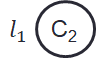
\includegraphics[scale=0.4]{empty}
	\end{subfigure}
	\vspace{5mm}
    
    \hspace{-10mm}
	\begin{subfigure}[t]{0.4\linewidth}\vskip 0pt
		\centering
		\caption{$\{a_1\}$}\label{fig:a1}
		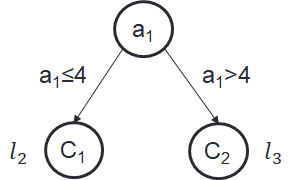
\includegraphics[scale=0.4]{a1}
	\end{subfigure}
	\quad
	\begin{subfigure}[t]{1in}\vskip 0pt
		\centering
		\caption{$\{a_2\}$}\label{fig:a2}
		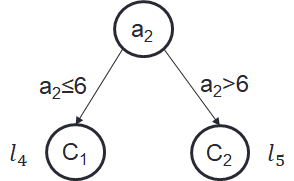
\includegraphics[scale=0.4]{a2}
	\end{subfigure}
	\quad
	\begin{subfigure}[t]{1in}\vskip 0pt
		\centering
		\caption{$\{a_3\}$}\label{fig:a3}
		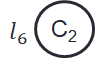
\includegraphics[scale=0.4]{a3}
	\end{subfigure}
	
	\vspace{5mm}
    \hspace{-10mm}
	\begin{subfigure}[t]{1in}\vskip 0pt
		\centering
		\caption{$\{a_1,a_2\}$}\label{fig:a1a2}
		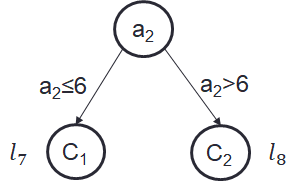
\includegraphics[scale=0.4]{a1a2}
	\end{subfigure}
	\quad
	\begin{subfigure}[t]{1in}\vskip 0pt
		\centering
		\caption{$\{a_1,a_3\}$}\label{fig:a1a3}
		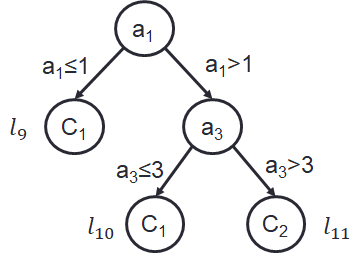
\includegraphics[scale=0.4]{a1a3}
	\end{subfigure}
	\quad
    \begin{subfigure}[t]{1in}\vskip 0pt
		\centering
		\caption{$\{a_2,a_3\}$}\label{fig:a2a3}
		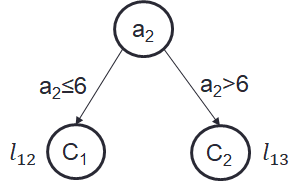
\includegraphics[scale=0.4]{a2a3}
	\end{subfigure}
	\quad
    
	\vspace{5mm}
    \hspace{-20mm}
	\begin{subfigure}[t]{1in}\vskip 0pt
		\centering
		\caption{$\{a_1,a_2,a_3\}$}\label{fig:a1a2a3}
		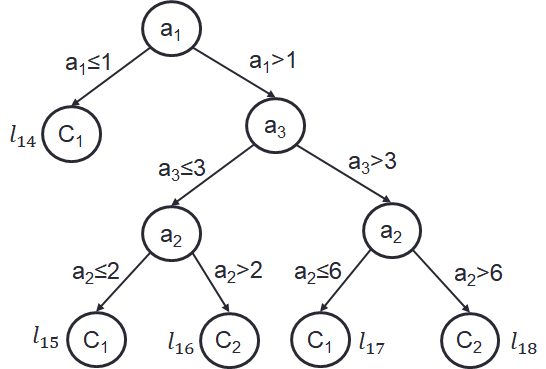
\includegraphics[scale=0.3]{a1a2a3}
	\end{subfigure}
	\caption{Constructed decision trees for all attribute subsets, constructed using the train data in Table~\ref{tbl:examples}.}\label{fig:Trees}
\end{figure}


\begin{figure}[ht]
\centering
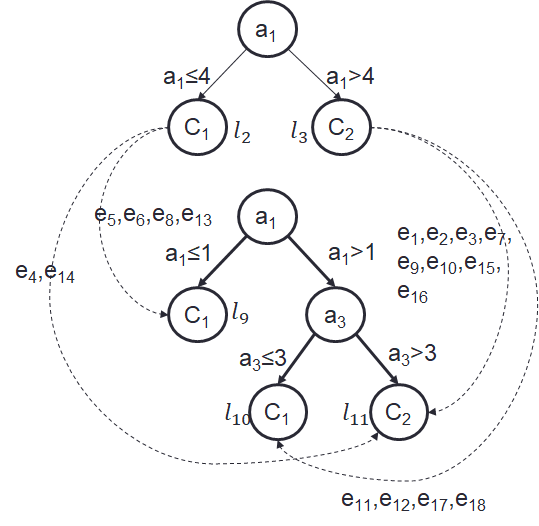
\includegraphics[scale=0.5]{Transition2}
\caption{Possible transitions from the leaves in $T_{\{a_1\}}$ to the leaves in the tree for $T_{\{a_1,a_3\}}$, using the test $a_3$ action.}
\label{fig:transition}
\end{figure}

Figure~\ref{fig:transition} provides an example of the transition from the leaves of the tree $T_{\{a_1\}}$, using the action $a_3$, revealing the value of the attribute $a_3$. The transition is hence to the leaves of the tree $T_{\{a_1,a_3\}}$. In this example $\tau(l_3,a_3,e_1)=l_{11}$, and $\tau(l_3,a_3,e_{11})=l_{10}$.



Let us further assume that the test cost for attribute $a_i$ is $i$, and symmetric misclassification cost for all classes of 10 (and a reward of 10 for successful classification). 

We can now begin computing the policy backward from the largest tree to the smaller ones. Looking at $T_{\{a_1,a_2,a_3\}}$, given symmetric misclassification costs it is always best to predict the most popular class in each leaf (specified in the leaves in Figure~\ref{fig:Trees}). 

Turning our attention now to $T_{a_1,a_3}$, the only available non-classification action is testing $a_2$. For $l_{11}$ we must compute the values using Equations~\ref{eqn:qlc} to ~\ref{eqn:pi}, where $E_{l_{11}} = \{e_1,e_2,e_3,e_4,e_7,e_9,e_{10},e_{14},e_{15},e_{16} \}$. We first compute the misclassification action value for $l_{11}$ using Equation~\ref{eqn:qlc}:
{\small
\begin{eqnarray}
pr(c_1|l_{11}) &=& \frac{4}{10} \\
pr(c_2|l_{11}) &=& \frac{6}{10} \\
Q(l_{11},c_1) &=& \frac{4}{10} \cdot 10 + \frac{6}{10} \cdot (-10) = -2\\
Q(l_{11},c_2) &=& \frac{6}{10} \cdot 10 + \frac{4}{10} \cdot (-10) = 2
\end{eqnarray}
}%
We now compute $Q(l,a)$ using Equation~\ref{eqn:qla}. Examples $e_4,e_{15},e_{16}$ transition to $l_{17}$, where they are classified as $c_1$, which is correct for $e_4,e_{15}$ but not for $e_{16}$. Examples $e_1,e_2,e_3,e_7,e_9,e_{10},e_{14}$ transition to $l_{18}$, where 5 of them are correctly classified as $c_2$, and two ($e_{7},e_{14}$) is misclassified. Computing $Q(l,a)$ we get:
\begin{equation}
\small
Q(l_{11},a_2) = -2 + \frac{5 \cdot 10 + 2 \cdot (-10) + 2 \cdot 10 + 1 \cdot (-10)}{10} = 2
\end{equation}
Hence, for $l_{11}$, $\argmax_{act \in \mathcal{A} \cup C} Q(l_{11},act) = c_2$ / $a_2$, so we are indifferent between classify as $c_2$ to test $a_2$ value. 

For the leaf $l_9$, all examples transition to leaf $l_{14}$, with the same class distribution. Hence:
{\small
\begin{align}
Q(l_{9},c_1) = Q(l_{14},c_1) &=& \frac{3}{4} \cdot 10 + \frac{1}{4} \cdot (-10) = 5\\
Q(l_9,a_2) &=& -2 + 5 = 3
\end{align}
}%
and therefore $\pi(l_9)=c_1$.

For $l_{10}$, $E_{l_{10}}=\{e_{11},e_{12},e_{17},e_{18} \}$, and the examples are evenly split between the classes, but after sensing the value of $a_2$, moving to $l_{15}$ and $l_{16}$, we improve the classification accuracy, misclassifying only a single example ($e_{12}$):
{\small
\begin{align}
Q(l_{10},c_1) &=& Q(l_{10},c_2) = \frac{2}{4} \cdot 10 + \frac{2}{4} \cdot (-10) = 0\\
Q(l_{10},a_2) &=& -2 + \frac{1 \cdot 10 + 2 \cdot 10 + 1 \cdot (-10)}{4} = 3
\end{align}
}%
and therefore $\pi(l_{10})=a_2$.








\section{Empirical Evaluation}

We now provide an experimental evaluation to compare our MDP-based cost sensitive classification method to other methods. We experiments with all domains from the recent cost sensitive survey \cite{LomaxV13,LomaxV11}, comparing our approach to the leading methods in the survey. 

\begin{figure}[!ht]
	\centering
	\begin{subfigure}[t]{0.5\textwidth}\vskip 0pt
		\centering
		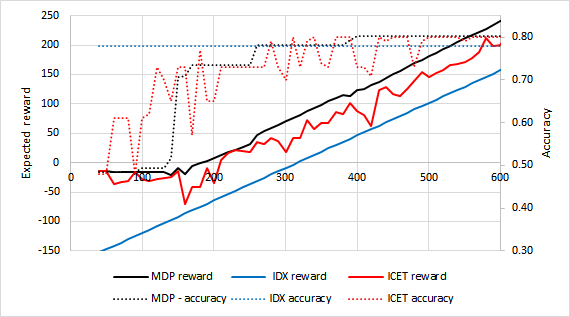
\includegraphics[scale=0.55]{Glass}
		\caption{Glass}\label{fig:Glass}		
	\end{subfigure}
    \quad
    
	\begin{subfigure}[t]{0.5\textwidth}\vskip 0pt
		\centering
		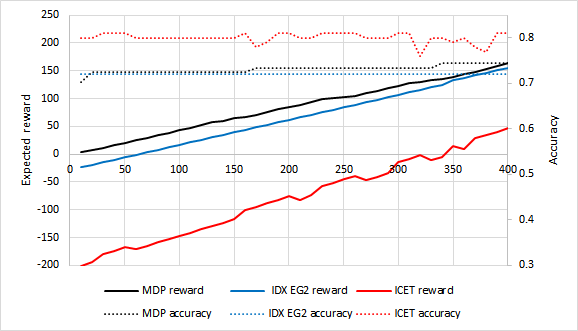
\includegraphics[scale=0.55]{Heart}
		\caption{Heart.}\label{fig:Heart}
	\end{subfigure}

    \caption{Comparing the expected reward and accuracy for varying misclassification costs (x-axis). In Heart, IDX and EG2 have identical performance and are reported together.}
    \label{fig:RewardVsAccuracy}
\end{figure}

\begin{table*}[t]
\centering
\scriptsize
\caption{Average classification reward (Rw) and average accuracy (Ac) with \underline{symmetric} ($r_{c,c}=-r_{c,c'}$) misclassification costs. $r_{c,c'}$ shows the varying misclassification cost that we use, and $\overline{r_a}$ is the average cost for testing an attribute. MDP is our approach. IDX, CSID3, EG2 are the modification of $C4.5$ to cost sensitive splits. $C4.5$ is the original, cost insensitive algorithm.}
\label{tbl:symmetric}
\npdecimalsign{.}
\nprounddigits{2}
\begin{tabular}{|c|c|c|c|c|c|c|c|c|c|c|c|c|c|c|c|c|}
\hline
&&& \multicolumn{2}{c|}{MDP}     & \multicolumn{2}{c|}{IDX} & \multicolumn{2}{c|}{CSID3}   & \multicolumn{2}{c|}{EG2} & \multicolumn{2}{c|}{C45}    & \multicolumn{2}{c|}{MetaCost} & \multicolumn{2}{c|}{ICET}    \\ \hline
Domain&$r_{c,c}$&$\overline{r_a}$&Ac&Rw&Ac&Rw&Ac&Rw&Ac&Rw&Ac&Rw&Ac&Rw&Ac&Rw \\ \hline

\multirow{3}{*}{\textbf{Car}}       & 10       & 43.12327 & 0.68  & \textbf{3.52}    & 0.96  & -128.49          & 0.98   & -136.11           & 0.96      & -128.79      & 0.96  & -137.49          & 0.96     & -137.57            & 0.68   & \textbf{3.52}    \\ \cline{2-17} 
                                    & 100      &          & 0.69  & \textbf{35.23}   & 0.96  & -46.19           & 0.98   & -50.14            & 0.96      & -46.49       & 0.96  & -54.82           & 0.96     & -54.91             & 0.93   & -47.00           \\ \cline{2-17} 
                                    & 300      &          & 0.96  & 129.45           & 0.96  & 136.70           & 0.98   & \textbf{140.89}   & 0.96      & 136.41       & 0.96  & 128.88           & 0.96     & 128.80             & 0.96   & 140.00           \\ \hline
\multirow{3}{*}{\textbf{Breast}}    & 100      & 41.71514 & 0.70  & \textbf{39.03}   & 0.85      & -94.21       & 0.84   & -112.21           & 0.85      & -94.21       & 0.85      & -121.35      & 0.86         & -173.10        & 0.79   & -38.78           \\ \cline{2-17} 
                                    & 400      &          & 0.91  & \textbf{222.11}  & 0.85      & 114.91       & 0.84   & 89.93             & 0.85      & 114.91       & 0.85      & 88.94        & 0.86         & 41.85          & 0.77   & 118.56           \\ \cline{2-17} 
                                    & 600      &          & 0.92  & \textbf{390.56}  & 0.85      & 254.33       & 0.84   & 224.68            & 0.85      & 254.33       & 0.85      & 229.14       & 0.86         & 185.15         & 0.82   & 230.01           \\ \hline

\multirow{3}{*}{\textbf{Hepatitis}} & 5        & 2.24     & 0.93  & \textbf{-0.07}   & 0.99      & -1.95        & 0.99   & -6.65             & 0.99      & -1.95        & 0.99  & -9.64            & 0.99     & -10.83             & 0.91    & -1.00           \\ \cline{2-17} 
                                    & 10       &          & 0.96  & \textbf{5.27}    & 0.99      & 2.92         & 0.99   & -1.79             & 0.99      & 2.92         & 0.99  & -4.77            & 0.99     & -5.96              & 0.92    & 1.30            \\ \cline{2-17} 
                                    & 30       &          & 0.98  & \textbf{27.47}   & 0.99      & 22.39        & 0.99   & 17.69             & 0.99      & 22.39        & 0.99  & 14.70            & 0.99     & 13.51              & 0.98    & 22.86           \\ \hline

\multirow{3}{*}{\textbf{Nursery}}   & 10       & 23.24092 & 0.42  & \textbf{-1.50}   & 0.97      & -119.12      & 0.98   & -109.81           & 0.98      & -118.81      & 0.98      & -109.40      & 0.98         & -110.29        & 0.42   & \textbf{-1.50}   \\ \cline{2-17} 
                                    & 100      &          & 0.66  & \textbf{-11.14}  & 0.97      & -33.90       & 0.98   & -22.84            & 0.98      & -32.96       & 0.98      & -22.35       & 0.98         & -23.18         & 0.48   & -18.40           \\ \cline{2-17} 
                                    & 150      &          & 0.98  & \textbf{18.70}   & 0.97      & 3.97         & 0.98   & 16.33             & 0.98      & 5.19         & 0.98      & 16.33        & 0.98         & 16.33          & 0.94   & 2.42             \\ \hline

\multirow{3}{*}{\textbf{Tictactoe}} & 5        & 1        & 0.64  & \textbf{1.36}    & 0.87  & -0.57            & 0.82   & -0.89             & 0.87      & -0.57        & 0.87  & -0.57            & 0.86     & -0.58              & 0.64   & \textbf{1.36}    \\ \cline{2-17} 
                                    & 10       &          & 0.84  & \textbf{4.70}    & 0.87  & 3.08             & 0.82   & 2.29              & 0.87      & 3.08         & 0.87  & 3.08             & 0.86     & 3.04               & 0.83   & 3.40             \\ \cline{2-17} 
                                    & 100      &          & 0.93  & \textbf{86.63}   & 0.87  & 68.84            & 0.82   & 59.56             & 0.87      & 68.84        & 0.87  & 68.84            & 0.86     & 68.19              & 0.83   & 62.00            \\ \hline
\multirow{3}{*}{\textbf{Wine}}      & 10       & 53.5927  & 0.68  & \textbf{-38.68}  & 0.95  & -141.54          & 0.99   & -163.93           & 0.98      & -148.00      & 0.99  & -183.30          & 0.99     & -183.30            & 0.98   & -189.43          \\ \cline{2-17} 
                                    & 100      &          & 0.91  & \textbf{13.41}   & 0.95  & -60.39           & 0.99   & -74.91            & 0.98      & -60.95       & 0.99  & -95.26           & 0.99     & -95.26             & 0.99   & -130.40          \\ \cline{2-17} 
                                    & 500      &          & 0.99  & \textbf{394.92}  & 0.95  & 300.26           & 0.99   & 320.72            & 0.98      & 325.93       & 0.99  & 295.99           & 0.99     & 295.99             & 0.99   & 265.50           \\ \hline


\end{tabular}
\end{table*}

\begin{table*}[t]
\centering
\scriptsize
\caption{Average reward (Rw) and average accuracy (Ac) \underline{asymmetric} misclassification costs. $r_{c,c'}$ shows the range from which misclassification costs were randomly selected, and $\overline{r_a}$ is the average cost for attribute testing. IDX, CSID3, EG2 are the modification of $C4.5$ to cost sensitive splits. $C4.5$ is the original, cost insensitive algorithm.}
\label{tbl:asymmetric}
\npdecimalsign{.}
\nprounddigits{2}
\begin{tabular}{|c|c|c|c|c|c|c|c|c|c|c|c|c|c|c|c|c|}
\hline
	&&& \multicolumn{2}{c|}{MDP}     & \multicolumn{2}{c|}{IDX} & \multicolumn{2}{c|}{CSID3}   & \multicolumn{2}{c|}{EG2} & \multicolumn{2}{c|}{C45}    & \multicolumn{2}{c|}{MetaCost} & \multicolumn{2}{c|}{ICET}    \\ \hline
Domain&$r_{c,c}$&$\overline{r_a}$&Ac&Rw&Ac&Rw&Ac&Rw&Ac&Rw&Ac&Rw&Ac&Rw&Ac&Rw \\ \hline

\multirow{3}{*}{\textbf{Car}}       & 15-45     & 43.12327  & 0.68  & \textbf{22.61}   & 0.95      & -103.72      & 0.97   & -110.49           & 0.95      & -104.01      & 0.96      & -112.60      & 0.96         & -112.55        & 0.68   & \textbf{22.61}   \\ \cline{2-17} 
                                    & 25-155    &           & 0.23  & \textbf{6.57}    & 0.96      & -74.25       & 0.97   & -79.73            & 0.96      & -74.54       & 0.95      & -81.62       & 0.95         & -82.78         & 0.68   & -7.84            \\ \cline{2-17} 
                                    & 300-480   &           & 0.96  & 176.15           & 0.95      & 182.34       & 0.97   & \textbf{188.92}   & 0.95      & 182.05       & 0.96      & 176.36       & 0.96         & 176.36         & 0.95   & 138.00           \\ \hline
\multirow{3}{*}{\textbf{Breast}}    & 350-400   & 41.71514  & 0.75  & \textbf{92.24}   & 0.74      & 12.01        & 0.72   & 32.11             & 0.74      & 12.01        & 0.74      & 44.03        & 0.74         & 45.29          & 0.73   & 37.14            \\ \cline{2-17} 
                                    & 350-450   &           & 0.76  & \textbf{212.04}  & 0.74      & 128.83       & 0.72   & 143.28            & 0.74      & 128.83       & 0.74      & 174.50       & 0.74         & 174.49         & 0.73   & 155.30           \\ \cline{2-17} 
                                    & 500-800   &           & 0.66  & \textbf{148.53}  & 0.74      & 42.19        & 0.72   & 65.99             & 0.74      & 42.19        & 0.74      & 81.21        & 0.74         & 82.46          & 0.75   & 94.10            \\ \hline

\multirow{3}{*}{\textbf{Hepatitis}} & 0-9       & 2.24      & 0.95  & \textbf{2.94}    & 0.99      & 1.13         & 0.99   & -3.58             & 0.99      & 1.13         & 0.99      & -6.56        & 0.98         & -6.51          & 0.94   & 1.50             \\ \cline{2-17} 
                                    & 0-20      &           & 0.97  & \textbf{9.00}    & 0.99      & 6.40         & 0.99   & 1.69              & 0.99      & 6.40         & 0.99      & -1.29        & 0.99         & -2.48          & 0.94   & 8.00             \\ \cline{2-17} 
                                    & 25-70     &           & 0.99  & \textbf{26.00}   & 0.99      & 19.11        & 0.84   & 10.84             & 0.99      & 19.11        & 0.96      & 11.64        & 0.98         & 7.40           & 0.99   & 23.00            \\ \hline
\multirow{3}{*}{\textbf{Nursery}}   & 0-70      & 23.24092  & 0.98  & \textbf{62.06}   & 0.97      & 44.36        & 0.98   & 58.58             & 0.98      & 46.95        & 0.98      & 58.85        & 0.98         & 46.95          & 0.94   & 44.27            \\ \cline{2-17} 
                                    & 10-130    &           & 0.59  & \textbf{46.32}   & 0.97      & 0.67         & 0.98   & 16.72             & 0.98      & 3.25         & 0.99      & 16.99        & 0.98         & 3.25           & 0.55   & 15.40            \\ \cline{2-17} 
                                    & 10-170    &           & 0.66  & \textbf{80.69}   & 0.97      & 40.52        & 0.98   & 55.62             & 0.98      & 42.87        & 0.98      & 56.01        & 0.98         & 42.87          & 0.53   & 53.00            \\ \hline
\multirow{3}{*}{\textbf{Tictactoe}} & 0-13      & 1         & 0.95  & \textbf{54.00}   & 0.87      & 45.44        & 0.82   & 41.31             & 0.87      & 45.44        & 0.87      & 45.44        & 0.86         & 45.58          & 0.83   & 44.00            \\ \cline{2-17} 
                                    & 13-25     &           & 0.82  & \textbf{6.28}    & 0.87      & 3.81         & 0.81   & 3.14              & 0.87      & 3.81         & 0.87      & 3.81         & 0.90         & 4.10           & 0.64   & 5.73             \\ \cline{2-17} 
                                    & 35-70     &           & 0.95  & \textbf{10.50}   & 0.87      & 8.17         & 0.82   & 6.45              & 0.87      & 8.17         & 0.87      & 8.17         & 0.87         & 8.17           & 0.83   & 7.65             \\ \hline
\multirow{3}{*}{\textbf{Wine}}      & 100-200   & 53.5927   & 0.94  & \textbf{83.70}   & 0.95      & 9.44         & 0.99   & 2.30              & 0.98      & 14.29        & 0.99   & -19.53          & 0.99     & -19.53             & 0.98   & -25.20           \\ \cline{2-17} 
                                    & 50-300    &           & 0.95  & \textbf{47.56}   & 0.95      & -32.20       & 0.99   & -39.17            & 0.98      & -29.04       & 0.99   & -60.73          & 0.99     & -60.73             & 0.99   & -94.10           \\ \cline{2-17} 
                                    & 70-500    &           & 0.92  & \textbf{184.78}  & 0.95      & 118.84       & 0.99   & 119.95            & 0.98      & 134.78       & 0.99   & 93.70           & 0.99     & 93.70              & 0.99   & 64.45            \\ \hline

\end{tabular}
\end{table*}


\begin{table}[t]
\centering
\scriptsize
\caption{Model construction time (sec.) for all methods. For our MDP approach we also report classification time.}
\label{tbl:time}
\begin{tabular}{|c|c|c|c|c|c|c|c|c|}
%\hline
%\multirow{2}{*}{Domain} & \multicolumn{2}{c|}{MDP}            & \multirow{2}{*}{IDX} & \multirow{2}{*}{CSID3} & \multirow{2}{*}{EG2} & \multirow{2}{*}{C45} & \multirow{2}{*}{MetaCost} & \multirow{2}{*}{ICET} \\ \cline{2-3}
%&\multicolumn{2}{c|}{MDP}&&&&&Meta& \\

\rot{Domain}  & \rot{MDP Classification} & \rot{MDP Construction} & \rot{IDX} &\rot{CSID3}&\rot{EG2}&\rot{C45}&\rot{MetaCost}&\rot{ICET}\\ \hline
Car	&0.29	&6.4	&0.015	&0.243	&0.022	&0.017	&0.004	&8	\\ \hline
Breast	&0.38	&8.81	&0.003	&0.122	&0.005	&0.003	&0.002	&4	\\ \hline
Hepati	&0.06	&45.86	&0.015	&0.247	&0.019	&0.018	&0.004	&6	\\ \hline
Nursery	&3.9	&100.4	&0.023	&0.34	&0.03	&0.03	&0.004	&50	\\ \hline
Tictac	&2.65	&95.73	&0.016	&0.265	&0.015	&0.015	&0.003	&8	\\ \hline
Wine	&0.01	&5.63	&0.003	&0.125	&0.006	&0.005	&0.003	&4	\\ \hline
\end{tabular}
\end{table}


\subsubsection{Methods}

We base our implementation on Weka~\cite{Weka}, except for ICET. The $C4.5$ algorithm that ignores costs provides an indication of the achievable accuracy, and an illustration on the expected cost when optimizing accuracy. We modified the Weka implementation of $C4.5$ to consider costs following 3 cost sensitive rules --- CS-ID3, IDX, EG2. All three originally consider only test costs, and we modified them to consider misclassification cost when making a classification decision in a leaf. We also use Weka's implementation of MetaCost \cite{domingos1999metacost}. In addition, we compare to ICET \cite{turney1995cost}, which showed the best performance in the survey \cite{LomaxV11}. ICET and MetaCost consider also the misclassification costs. 

The experiments were run on a Windows 10 machine, $i5$ CPU, and 8GB RAM. Our method is implemented in $C\#$, ICET is implemented in C over a Linux virtual machine, and all other methods except for ICET are implemented in Java.


\subsubsection{Procedure}

The ratio between the test costs and misclassification costs results in different behaviors. When the misclassification cost is much lower than the test costs, executing any tests results in suboptimal behavior. When the misclassification cost, at the other extreme, is much larger than test costs, it is often better to execute all informative tests. Hence, the behavior is most interesting in between.

We therefore experiment in each domain with 3 selected misclassification costs --- one that is on the same order of the test costs, encouraging the algorithm to classify before executing many tests, one where the misclassification cost is sufficiently high to encourage the algorithm to execute many tests, and one where the misclassification cost is in between the two extremes. While we vary the misclassification costs we keep the test costs constant, as specified by Lomax and Vadera \shortcite{LomaxV11}. MDP, ICET and MetaCost that consider misclassification costs during construction were trained separately for each classification cost matrix.

We use a standard $80\%-20\%$ train-test split. Results are paired, that is, all algorithms were run on the same split. Dataset statistics are reported in Table~\ref{tbl:datasets}. For the larger datasets --- Heart, Wine and Hepatitis, we learned decision trees only over subsets of the 10 most costly attributes together with the low cost attributes.

Due to the lack of space, we present here just a part of the results. Complete tables and all graphs can be found in the supplementary material, showing that our method performs well over all domain and over a wide cost range.

\begin{table}[ht]
\centering
\footnotesize
\begin{tabular}{|c|c|c|c|}
\hline
 	Domain & Attributes&	Train	&Test \\ \hline
Iris&	4&	500&	250\\
Car&	6	&700&	300\\
 	 	 	 
 	 	 	 
%Diabetes&	7&	550&	250\\
 	 	 	 
%Flare&	10&	500	&200\\
 	 	 	 
Glass&	8&	500	&200\\
 	 	 	 
 	 	 	 
 	 	 	 
 	 	 	 
Nursery&	8&	6500&	2500\\
 	 	 	 
Tictactoe&	9&	700&	300\\
Breast&	9&	300&	100\\
 	 	 	 
Heart&	12&	200	&100\\
Wine&	13&	400&	200\\ 
Hepatitis&	17&	700&	300\\\hline

\end{tabular}
\caption{Dataset statistics}
\label{tbl:datasets}
\end{table}

\subsubsection{Results}

We first experiment with symmetric rewards and costs, that is, the cost of a misclassification is the negative of the reward for a successful classification. We also assume here that all misclassifications have the same cost. 
Symmetric misclassification costs are convenient for all methods (including ours) that ignore these costs when constructing the trees, as for symmetric costs, accuracy is completely correlated with the misclassification cost.



Table~\ref{tbl:symmetric} shows the average reward per classification, and the prediction accuracy for each classification method, given varying misclassification costs. It is obvious that the MDP approach has a much better reward than any other method, often sacrificing accuracy to achieve better reward. For medium misclassification costs, which arguably require the most sophisticated balancing of accuracy and cost, our method is always best. It is also always best at the extremes, except for one domain (Car).

$C4.5$ is almost never best. It is obviously worst at low misclassification costs, when running multiple test is not worthwhile. It is also not good when the misclassification costs are high, and all attributes are tested, because it does not order the tests with respect to the cost. 
The cost-sensitive algorithms based on $C4.5$ work well when misclassification costs are high, but preform badly when costs are low, and are also far from optimal for the medium costs.

Considering accuracy, ICET and MDP have reduced accuracy when the misclassification cost is low, because it is not worthwhile to test more attributes in order to improve accuracy. It is interesting to see, though, that the MDP method often has better accuracy than even $C4.5$, when the misclassification costs are sufficiently high to warrant expensive tests for improving accuracy. This is most pronounced on tictactoe, but occurs in other domains as well. We attribute the high accuracy to the MDP ability to consider all future tests, while $C4.5$ is making greedy decisions at each split.

Figure~\ref{fig:RewardVsAccuracy} compares the behavior of our MDP approach, ICET, and C4.5 methods as the misclassification costs (and rewards) increase. C4.5 based methods (IDX and EG2) ignore these costs, and hence maintain fixed accuracy. ICET fluctuates for different costs, which is typical for local search methods that often get stuck at local maxima. In Glass ICET is sometimes only slightly below the MDP. In Heart ICET finds a tree with excellent accuracy, but very low expected reward. IDX offers very low expected cost in Glass, but converges towards our MDP approach in Heart, when the misclassification costs are high, because in these cases it is advantageous to invest in additional testing for improving accuracy. The MDP accuracy curve contains several thresholds where the MDP policy changes to test more attributes, resulting in a significant increase in accuracy. 

We also experimented with asymmetric misclassification costs. We choose the costs and rewards uniformly from 3 ranges --- small, medium, and large --- all with respect to the test costs, as above. Table~\ref{tbl:asymmetric} shows these results for the asymmetric costs. Here, our MDP approach is almost always the best method. All other methods, while performing well in some cases, perform very poorly in other domains. For example, ICET does well on hepatitis, but does not perform well on breast. Overall, this table demonstrates, again, the superiority of our MDP approach over all other methods in most cases. MetaCost does much better on the asymmetric than the symmetric misclassification costs, and is sometimes better than ICET, but is best only rarely.

Table~\ref{tbl:time} shows the model construction time of the various methods. As can be expected, ICET takes much longer than the C4.5 methods, and our MDP approach takes the longest. In classification, all methods that use a single tree operate very rapidly, while our approach that recomputes the MDP policy after each test (Section~\ref{sec:RefineMDP}) is significantly slower. Still, in many applications, such as medical diagnosis, spending a few minutes constructing the model, and a few seconds during classification is reasonable, given the considerable improvement in expected reward.



\section{Conclusion}

In this paper we have suggested an MDP-based approach to cost sensitive classification, considering both test costs and misclassification costs. The MDP approach provides a sound method for reasoning about future actions, instead of considering only the myopic value of information. 

We construct standard decision trees over all attribute subsets, and the leaves of these trees become the state space of our MDP. We explain how transition probabilities can be estimated from the data, and define the costs and rewards of the MDP. We explain how our method enforces the Markovian property, and how the value iteration algorithm can be augmented to take our relaxation into consideration.

We analyze the sensitivity of our MDP method for test-misclassification cost ratios, and to symmetric and asymmetric costs. We provide extensive comparison with all methods and all domains from \cite{LomaxV11}, showing that our MDP approach is almost always best. 

In the future we intend to replace the naive creation of the decision trees with a method that takes into consideration the misclassification costs during tree construction. We also intend to investigate POMDPs instead of MDPs, as a better method for modeling the value of information.

\paragraph{\bf Acknowledgments:} Supported by ISF Grant 933/13, by the Helmsley Charitable Trust through the Agricultural, Biological and Cognitive Robotics Center, and by the Lynn and William Frankel Center for Computer Science.

%\pagebreak
\bibliographystyle{aaai}
\bibliography{biblio}
\end{document}




